\section*{Sources of bias in the SQF data}
\begin{figure}
    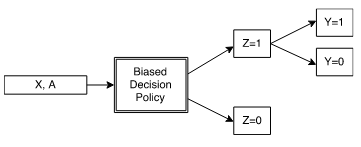
\includegraphics[width=0.7\textwidth]{../figures/selection_bias.png}
    \caption{Selection bias in the SQF data.}
    \label{fig:selection_bias}
\end{figure}
The major concern that has been identified in the literature for SQF data is how the data is generated in the first place. In their paper "Residual Unfairness" \cite{kallus} conceptualise the problem as shown in \autoref{fig:selection_bias}.
We define a person by their sensitive feature (A) and non-sensitive features (X). For each person in the population of interest a police officer decides whether to stop them or not. Based on this biased decision policy people are included in the sample (Z = 1) or they are not (Z = 0). But naturally we only observe further information on the people that were stopped. Only for them we can know the outcome of a stop, which constitutes the target of a classificaiton task.
\cite{kallus} distinguish between target population and training population in such scenarios. The target population is the one on which we want to use the ADM on while the training population are the observations the biased decision policy chose to include in the sample and on which the algorithm is trained.
In the SQF data we can see this form of bias by comparing the race distribution of NYC to the race distribution in the SQF data. From \autoref{fig:race_distributions} it is clear that in terms of race the SQF data does not represent the general population of the city. We can see that white people form the majority of the population in NYC, but only make up a tiny fraction of SQF stops. Black people in contrast are the third-largest ethnic group in NYC while they exceed any other group in the SQF data by far.
\autoref{fig:race_distributions} shows that selection bias might be at play in the decision of stopping a suspect.
\begin{figure}
    \centering
    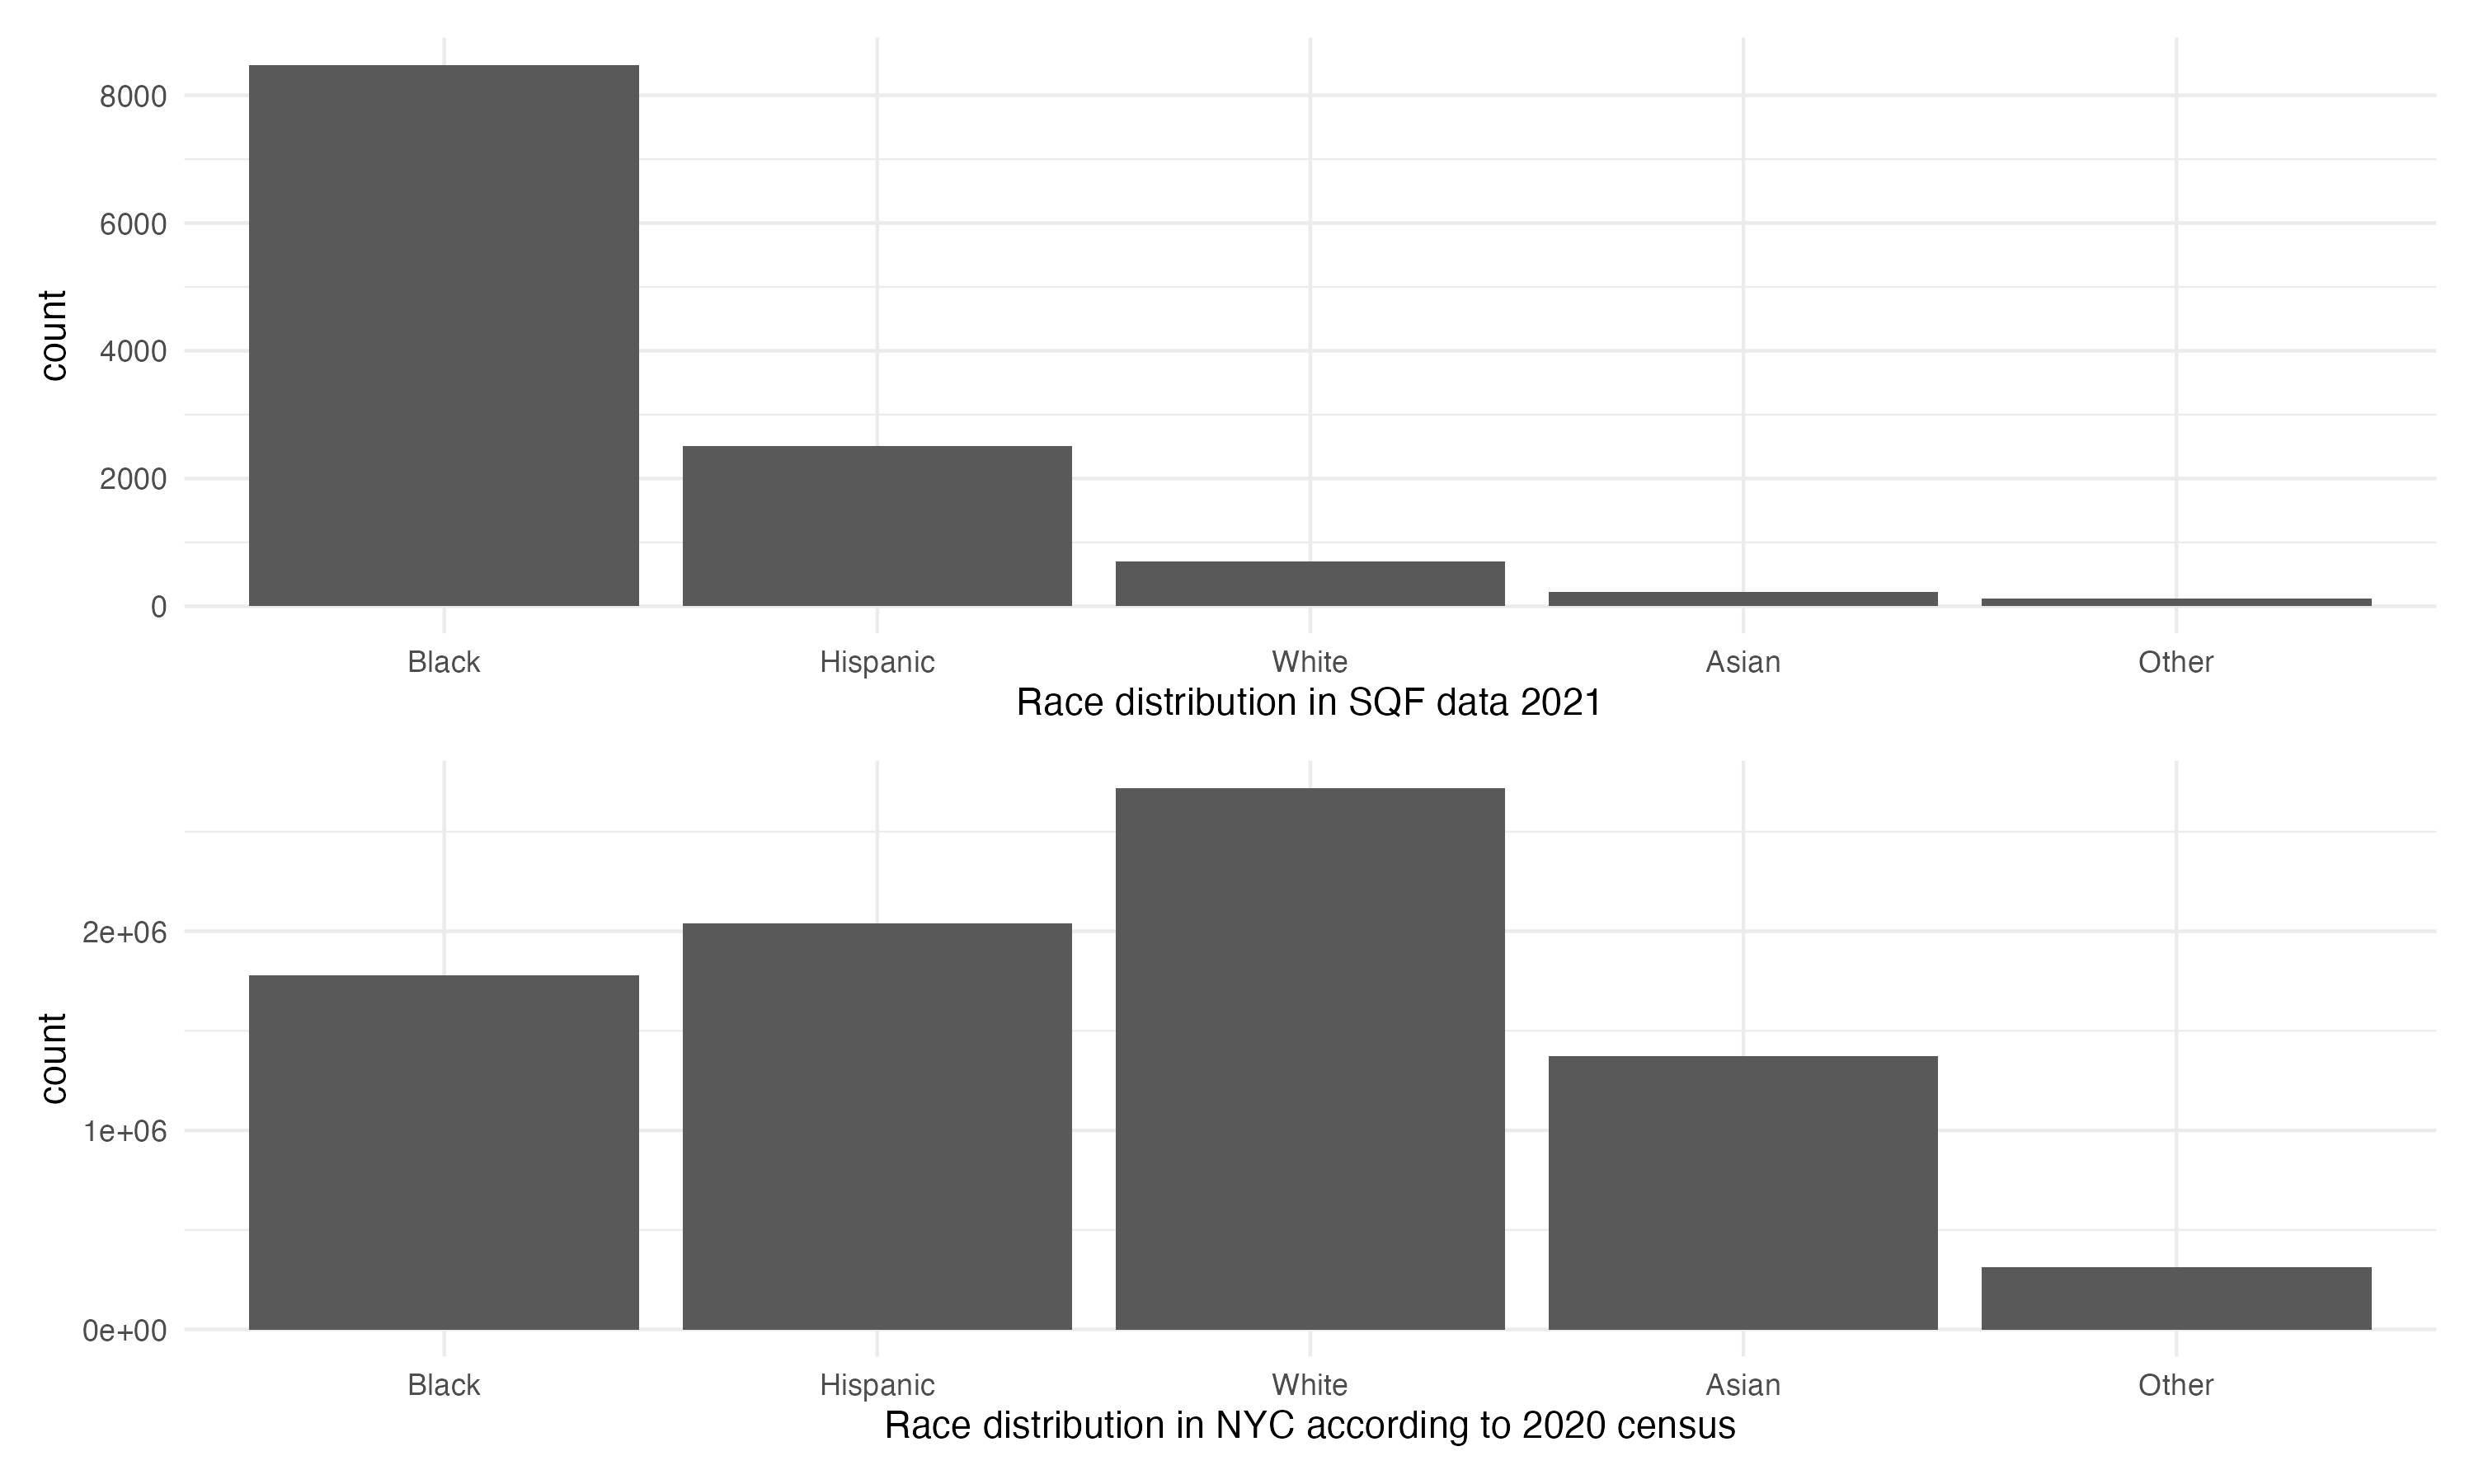
\includegraphics[width=0.7\textwidth]{../figures/sqf_case_study_plot6.png}
    \caption{Comparison of race distribution in the training and target population.}
    \label{fig:race_distributions}
\end{figure}

To get a more nuanced picture we also plot the true arrestment rate per ethnic group in the SQF 2023 data and find that White and Asian people have the highest arrestment rates and black people the lowest. This supports the argument that black people are stopped more leniently and there is a biased decision policy in place. The questions now are why the group metrics did not detect any unfairness in our algorithm and how such biases can be addressed in fairness practice.
% The main message of this paper is that it is not that easy to adjust for fairness, when the data the algorithm learns from is biased. Ensuring Equal Opportunity or Equalized Odds on the training data does not generalize to the target population. The paper proposes a way to estimate the TRP and FPR in the target population. This is useful, when the fairness methods depends on the FPR and/or TPR. 
Why the group metrics did not show any unfairness in the algorithm can be answered ins a straight forward way. Group metrics offer a rather isolated view on fairness. They assess disparities in algorithimic predictions between protected groups rather than measuring the fairness of a whole situation. Thus, group metrics are not designed to detect selection bias. They work with the joint distribution of $Y, A, X, \hat{Y}$ and do not take any additional information into account. When we rely on the true label $Y$ (Separation) to detect unfairness but the true label itself is not reliabel (generated via an objective truth), then the group metrics cannot show this \cite{castelnovo2022}.
To answer the second question we use the following chapter to examine two papers that propose methods to address selection bias in fairness practice and have explicity used the SQF data as a case study.

\section{Residual Unfairness}
We already outlined the formal problem setting in \cite{kallus} in \autoref{fig:selection_bias}. The main message of the paper supports the saying "bias in, bias out". They argue that fairness adjustments on the training population do not ensure fairness in the target population. Fairness is defined via equal opportunity or equalised odds. They propose to modify a post-processing method to deal with selection bias.

% Notation and problem setting
The paper uses the following notation: $A$ is the binary sensitive attribute, $X$ are the non-sensitive attributes, $Y$ is the target, $\hat{Y}$ is the prediction, $Z$ is the decision of the biased inclusion policy ($Z= 1$ means the subject is included into the training population). $T$ indicated whether a person is in the target population ($T = 1$) means that we want to use the trained algorithm on the person. $\hat{R} \in [0,1]$ is the prediction score.
The problem depicted in \autoref{fig:selection_bias} can be now expressed as follows. We only have knowledge about $X, A, Y | Z = 1$ while we do not know $X, A, Y | Z = 0$. 

% Fairness definition
The paper defines fairness via equal opportunity or equalised odds. Recall that equal opportunity demands that the false positive rate is the same across groups, i.e. $P(\hat{Y} = 0 | Y = 1, A = a) = P(\hat{Y} = 0 | Y = 1, A = b)$. But requiring equal false negative rates across groups is the same a requiring equal true positive rates across groups since $P(\hat{Y} = 0 | Y = 1, A = a) = 1 - P(\hat{Y} = 1 | Y = 1, A = a)$.
The paper uses a thresholding classifier, if the prediction score exceeds a certain threshold the positive value for the target is predicted. This allows us express the false negative rate and the true positive rate of a group $a$ with respect to an event $E$ via the cummulative distibution function. $F_a^E = P(\hat{R} \leq \theta | Y = 1, A = a, E)$. Note that we condition on the truly positive subject in the sample. In the SQF case this would mean that we only look at people that were truly arrested.
The truly arrested that have a predicted probability $\hat{R} \leq \theta$ are wrongly classified as not-arrested, while the ones for whom $\hat{R} > \theta$ are correctly classified as arrested. $F_a^Z$ gives us nothing other than the false negative rate in the training population and $F_a^T$ is the false negative rate in the target population.
So when we want to define an equal opportunity classifier on the training population we require $F_a^Z(\theta_a) = F_b^Z(\theta_b)$ to hold. 

% Definition of fair classifier 
An optimal derived equal opportunity classifier can then be defined as $\hat{Y} = I(\hat{R} > \theta_A)$ and $F_a^Z(\theta_a) = F_b^Z(\theta_b)$ for all groups a,b. In words, the classifier predicts the positive outcome with a group-specific threshold for each member of the group while this group specific threshold is set in such a way that equal opportunity on the training data is fulfilled. We will not go into detail of how one finds such a classifier but refer to \cite{hardt2016} who propose a post-processing method to derive the optimal thresholds for each group. 

With the definition of fairness as equal opportunity (equal tpr/fnr across groups) we can in turn define unfairness as inequity of opportunity. This describes nothing other than the difference in true positive rates between groups, i.e. \(\epsilon_{a,b}^E = P(\hat{Y} = 1 | Y = 1, A = a, E) - P(\hat{Y} = 1 | Y = 1, A = b, E)\). $\epsilon_{a,b}^{T=1} > 0$ shows discrimination against group b, since this means that the true positive rate for group b is lower than for group a.
When we construct an equal opportunity classifier (via some fairness intervention) then $\epsilon_{a,b}^{Z=1} = 0$ holds for this classifier. This also means that any inequity of opportunity that might show in the target population cannot be explained via existing ineuqities between groups in the training population but via existing differences in the training and the target population. So it is unfairness that gets introduced when we try to generalize our algorithm to the population it was not trained on. \cite{kallus} call this residual unfairness, since this is unfairness remaining event after fairness adjustments.

% Scenarios of discrimination
\subsubsection*{Strong disparate benefit of the doubt}
To fully understand the results of the paper, we additionally introduce the concept of stochastic dominance, originating from decision theory. Let $F, G$ be two cummulative distribution functions. Then $G$ first order stochastically dominates $F \preceq G$ when $F(\theta) \geq G(\theta)$ $\forall\theta$. Recall that G and F are cummulative distribution functions. So first order stochastic dominance of G over F, smaller values of G for each input value $\theta$, that the population described by the CDF of G consistently has higher probability values than population F. Their probability mass is concentrated towards the higher input values thus the cummulative distribution function is small for small input values.
Equipped with these definitions the paper constructs difference scenarios of (un)fairness. The bottom line always is that equal opportunity in the training population does not guarantee equal opportunity in the target population.

% Scenario 1: Strong disparat benefit of the doubt (Prop. 2)
For the first discrimination scenario we assume the following:
$F_a^{Z=1} \preceq F_a^{T=1} and F_a^{Z=1} \succeq F_a^{T=1}$ and at least one of the equalities does not hold (either $F_a^{Z=1} \ne F_a^{T=1}$ or $F_b^{Z=1} \ne F_b^{T=1}$ or both).
In words this means for group a, the target population first order stochastically dominates the training population. The truly positive individuals in group a consistently have lower scores than the ones in the target population. The score is the predicted probability of receiving the positive outcome. When for group a we have more people with low probabilites for the favourable outcome in our sample, then this means that group a member were more leniently introduced into the sample. The paper says that group a members recevied more "benefit of the doubt".
For the SQF scenario we reverse things. $\hat{Y} = 1$ is no longer desirable and we can interpret scores as riskscores $G_g^{E}$. So the score describes the probability for receiving the undesirable outcome. The proposition can be reformulated by switching the order signs.
Suppose that $G_a^{Z=1} \preceq G_a^{T=1}$ and $G_b^{Z=1} \preceq G_b^{T=1}$ while at least one of the equalities does not hold i.e. $G_a^{Z=1} \ne G_a^{T=1}$ or $G_b^{Z=1} \ne G_b^{T=1}$ or both. Then every derived equal opportunity classifier has nonnegative inequity of opportunity for group b relative to group a $\epsilon_{a,b}^{T=1} \geq 0$ and at least one derived equal opportunity classifier will have a strictly positive inequity of opportunity disadvantaging group b relative to group a $\epsilon_{a,b}^{T=1} > 0$.
In the context of SQF this means that group a members were stopped more carefully while group b members were stopped leniently. This aligns with the fact that the sqf data records considerably more stops for black people than white people. In this case the propositions of the paper will show us again that even after adjusting for equal error rates, the classifier will disadvantage group b when applied to the target population.


When we employ the algorithm in the target population, group a member will receive the positive outcome
 more easily (receive benefit of the doubt) because the thresholds is so low. For group b
 the opposite is true. The scores in the training data are really high compared to the overall population.
 This means we learn a high threshold for group b. When the system is applied on the whole population it will
 be harder for a random person from group b to receive the advantage because their threshold is so high.
Applied on the SQF data this could translate as follows. First of all, the interpretation shifts. $\hat{Y} = 1$ is 
no longer desirable and we can interpret scores as riskscores $G_g^{E}$. This means a high thresholds for being classified as $\hat{Y} = 1$ is desirable, a low
threshold is undesirable. We assume that officers were more lenient to stop black individuals, which means that the scores (probability of actually having committed crime) in the training population
of black people are lower than the scores of the target population of black people $G_b^{Z=1} \preceq G_b^{T=1}$.



When we apply the algorithm to the target population we will be more likely to classify black people as $\hat{Y} = 1$ because the threshold is so low. White people, on the other hand,
were selected more strictly. This means that the scores of white people in the training population are higher than the scores of white people in the target population.
$G_w^{Z=1} \succeq G_w^{T=1}$. This means we will learn a high threshold for white people. When we apply the algorithm to the target population we will be less likely to classify white
people as $\hat{Y} = 1$ because the threshold is so high. -- Still unsure if this makes sense, if a transfered it correctly.

For the other group we have many truly guilty and less truly innocent. When now 80\% of truly guilty are classified as guilty in the advantaged group then we would want want 80\% of
the truly guilty to be correctly labelled as guilty in the disadvantaged group. This would only results in lowering the threshold for the disadvantaged group
(so making it easier to predict them as guilty) if we predicted low risk scores for truly guilty people in the disadvantaged group
 Because for equal opportunity we are only looking at the people who were really guilty. So we are basically saying that the large proportion of truly
 innocent people in our sample of the disadvantaged leads to lower risk scores even in the truly guilty group of the disadvantaged (like a spill over effect).
 Only then it would make sense to say that a fairness intervention would compensate by setting lower thresholds for the disadvantaged group. Is this happening? 

Chapter 6: Case study on SQF data
Their main message is always, bias in, bias out. fairness interventions, done on the training data are not enough, if your sample is biased, your model will be biased (even after fairness interventions).
They show this in the following way. The goal is to predict innocence of an individual. Such an ADM could help officers
decide who to stop in the first place. The SQF data serves as training data and is naturally censored. The censoring process is that we only
observe innocence of a person if they were stopped. But the decision to stop someone could be based on a biased decision policy.
So we have our censored training data (SQF data). We know that this training data is not representative of the population of NYC in general defined via
location specific variables. Kallus and Zhou use train a logistic regression classifier on the SQF data as is and use post-processing proposed
by Hardt et al. to ensure Equal Opportunity or Equalized Odds. They use their a weighing technique (proposed by them and inspired by propensity score matching)
to simulate the target population. The fairness intervention in the training population produces group-specific thresholds that are then applied to the target population.
They use these fairness-adjusted threshold for the target population and still observe unfairness.

But of course they observe unfairness because the fairness intervention they do is a post-processing step and doesn't modifiy the classifier. What am i not getting here?